\documentclass[10pt]{article}
\usepackage{fontspec}
\setmainfont{lmroman10-regular.otf}[BoldFont=lmroman10-bold.otf,ItalicFont=lmroman10-italic.otf,BoldItalicFont=lmroman10-bolditalic.otf]
\setmonofont{lmmono10-regular.otf}
\usepackage[a4paper,margin=16mm,top=14mm,bottom=16mm]{geometry}
\usepackage{multicol,graphicx,xcolor,array,fancyhdr}
\usepackage[hidelinks]{hyperref}
\setlength{\columnsep}{6mm}
\setlength{\parindent}{1em}
\setlength{\parskip}{2pt}
\newcommand{\unk}[1]{\textcolor{red}{\texttt{\scriptsize[U+#1]}}}
\pagestyle{fancy}\fancyhf{}\renewcommand{\headrulewidth}{0.4pt}
\fancyhead[C]{\small HELMINTHOLOGY. Plate CCLI}
\fancyfoot[C]{\scriptsize Sthold Owner Walls Instagram from}
\begin{document}
% block 3 Picture bbox=[0.0977, 0.0773, 0.9004, 0.3125]
\begin{center}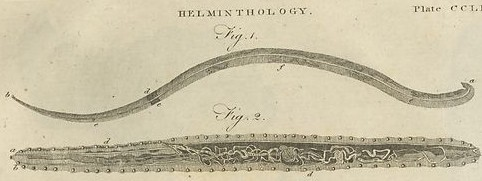
\includegraphics[width=\linewidth,height=0.45\textheight,keepaspectratio]{img/651-3.jpg}\end{center}
{\scriptsize\color{gray}\noindent Text inside picture (Parse): Fig.2.\par}
\begin{multicols}{2}\raggedcolumns
% block 1 Caption bbox=[0.4502, 0.1078, 0.5215, 0.1391]
\begin{center}\small\itshape Fig 1\end{center}
% block 2 Caption bbox=[0.4492, 0.2094, 0.542, 0.2437]
\begin{center}\small\itshape Fig.2.\end{center}
% block 4 Caption bbox=[0.4453, 0.3359, 0.543, 0.3695]
\begin{center}\small\itshape Fig.1.\end{center}
% block 5 Picture bbox=[0.0879, 0.4797, 0.2939, 0.643]
\begin{center}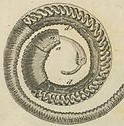
\includegraphics[width=\linewidth,height=0.45\textheight,keepaspectratio]{img/651-5.jpg}\end{center}
{\scriptsize\color{gray}\noindent Text inside picture (Parse): O\par}
% block 6 Picture bbox=[0.5928, 0.4133, 0.9053, 0.5406]
\begin{center}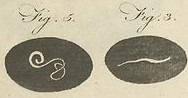
\includegraphics[width=\linewidth,height=0.45\textheight,keepaspectratio]{img/651-6.jpg}\end{center}
{\scriptsize\color{gray}\noindent Text inside picture (Parse): Fig.3. Fig.3.\par}
% block 7 Picture bbox=[0.6094, 0.5461, 0.8896, 0.6523]
\begin{center}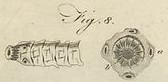
\includegraphics[width=\linewidth,height=0.45\textheight,keepaspectratio]{img/651-7.jpg}\end{center}
{\scriptsize\color{gray}\noindent Text inside picture (Parse): Fig.8.\par}
% block 8 Caption bbox=[0.4336, 0.6766, 0.5322, 0.7141]
\begin{center}\small\itshape Fig.7.\end{center}
\end{multicols}
% block 9 Picture bbox=[0.1045, 0.7094, 0.9111, 0.7781]
\begin{center}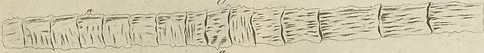
\includegraphics[width=\linewidth,height=0.45\textheight,keepaspectratio]{img/651-9.jpg}\end{center}
{\scriptsize\color{gray}\noindent Text inside picture (Parse): Fig.9.\par}
\begin{multicols}{2}\raggedcolumns
% block 10 Caption bbox=[0.4375, 0.7891, 0.5342, 0.8273]
\begin{center}\small\itshape Fig.9.\end{center}
\end{multicols}
\vfill\par\noindent\rule{\linewidth}{0.4pt}\par
{\scriptsize\color{gray}\noindent Source: Encyclopaedia Britannica scan, text from Parse 3.5 without correction. page\_id: britannica:309f765b1ecc83e0a7f7762e44b4a927a7555443:train:651 \quad row index: 651 \quad image sha256: a4e89a900a4041b934828dcc5c677df6edf0de903ab97d097948b7b17427da7d \quad parse model: nvidia/nemotron-3.5-parse \quad parse finish: stop \quad scan: \href{../scans/page-0651-a4e89a900a40.jpg}{page-0651-a4e89a900a40.jpg}\par}
\end{document}
